% Created by tikzDevice version 0.12.6 on 2024-04-17 08:38:48
% !TEX encoding = UTF-8 Unicode
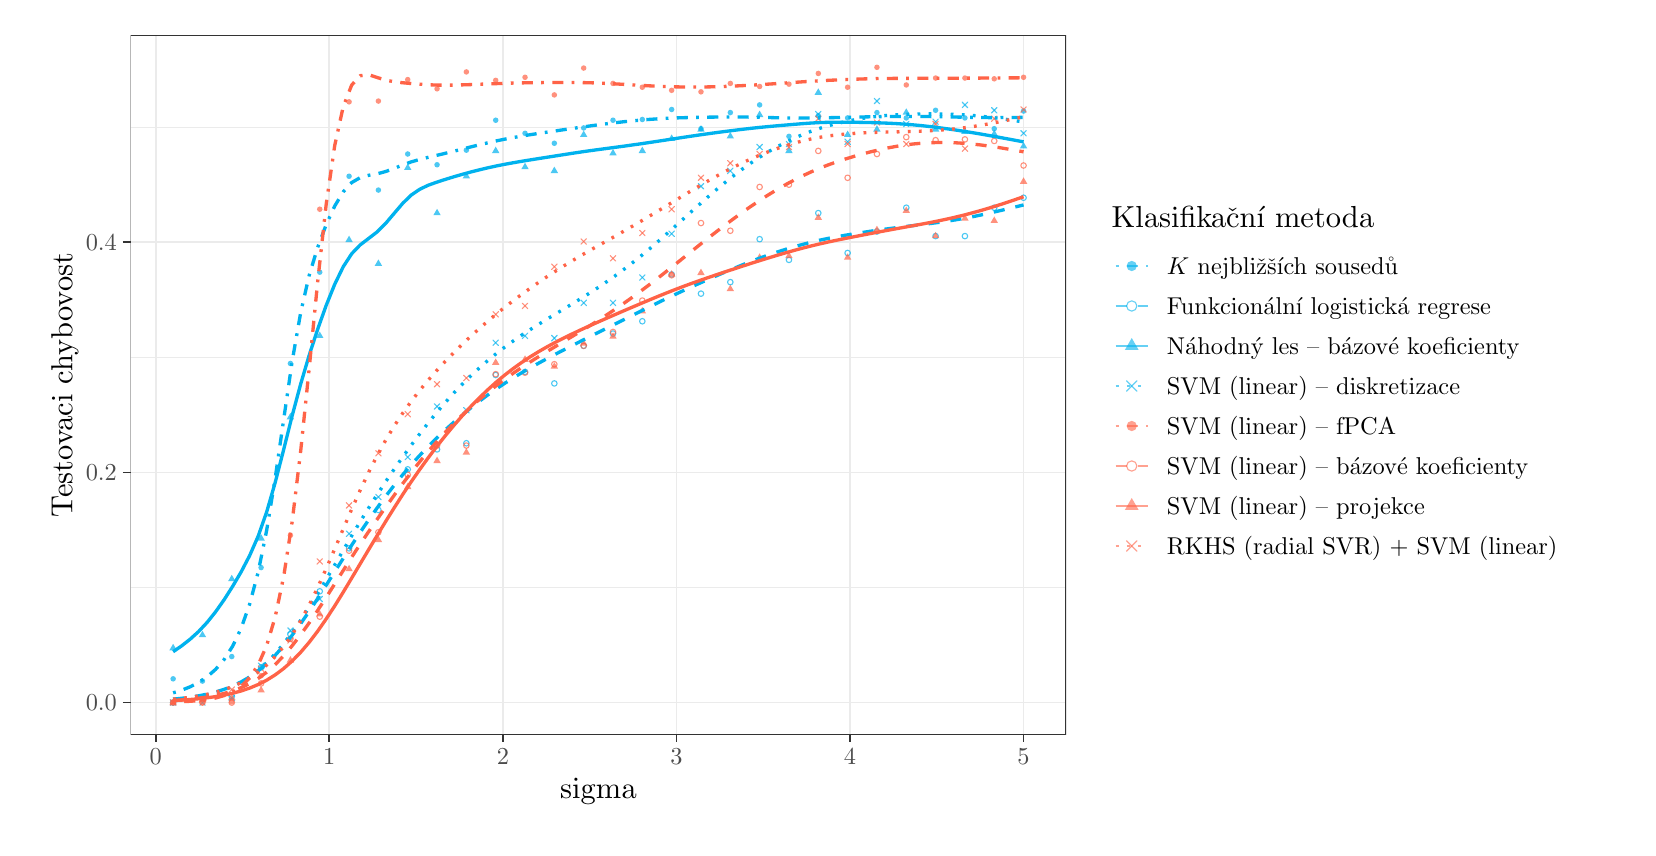
\begin{tikzpicture}[x=1pt,y=1pt]
\definecolor{fillColor}{RGB}{255,255,255}
\path[use as bounding box,fill=fillColor] (0,0) rectangle (578.16,289.08);
\begin{scope}
\path[clip] (  0.00,  0.00) rectangle (578.16,289.08);
\definecolor{drawColor}{RGB}{255,255,255}

\path[draw=drawColor,line width= 0.6pt,line join=round,line cap=round,fill=fillColor] (  0.00,  0.00) rectangle (578.16,289.08);
\end{scope}
\begin{scope}
\path[clip] ( 37.19, 33.72) rectangle (375.23,286.23);
\definecolor{fillColor}{RGB}{255,255,255}

\path[fill=fillColor] ( 37.19, 33.72) rectangle (375.23,286.23);
\definecolor{drawColor}{gray}{0.92}

\path[draw=drawColor,line width= 0.3pt,line join=round] ( 37.19, 86.79) --
	(375.23, 86.79);

\path[draw=drawColor,line width= 0.3pt,line join=round] ( 37.19,169.96) --
	(375.23,169.96);

\path[draw=drawColor,line width= 0.3pt,line join=round] ( 37.19,253.13) --
	(375.23,253.13);

\path[draw=drawColor,line width= 0.6pt,line join=round] ( 37.19, 45.20) --
	(375.23, 45.20);

\path[draw=drawColor,line width= 0.6pt,line join=round] ( 37.19,128.37) --
	(375.23,128.37);

\path[draw=drawColor,line width= 0.6pt,line join=round] ( 37.19,211.55) --
	(375.23,211.55);

\path[draw=drawColor,line width= 0.6pt,line join=round] ( 46.29, 33.72) --
	( 46.29,286.23);

\path[draw=drawColor,line width= 0.6pt,line join=round] (109.00, 33.72) --
	(109.00,286.23);

\path[draw=drawColor,line width= 0.6pt,line join=round] (171.72, 33.72) --
	(171.72,286.23);

\path[draw=drawColor,line width= 0.6pt,line join=round] (234.43, 33.72) --
	(234.43,286.23);

\path[draw=drawColor,line width= 0.6pt,line join=round] (297.15, 33.72) --
	(297.15,286.23);

\path[draw=drawColor,line width= 0.6pt,line join=round] (359.86, 33.72) --
	(359.86,286.23);
\definecolor{fillColor}{RGB}{0,178,238}

\path[fill=fillColor,fill opacity=0.70] ( 52.56, 53.79) circle (  1.00);

\path[fill=fillColor,fill opacity=0.70] ( 63.15, 52.96) circle (  1.00);

\path[fill=fillColor,fill opacity=0.70] ( 73.75, 61.83) circle (  1.00);

\path[fill=fillColor,fill opacity=0.70] ( 84.35, 93.99) circle (  1.00);

\path[fill=fillColor,fill opacity=0.70] ( 94.94,167.74) circle (  1.00);

\path[fill=fillColor,fill opacity=0.70] (105.54,200.73) circle (  1.00);

\path[fill=fillColor,fill opacity=0.70] (116.14,235.39) circle (  1.00);

\path[fill=fillColor,fill opacity=0.70] (126.73,230.40) circle (  1.00);

\path[fill=fillColor,fill opacity=0.70] (137.33,243.43) circle (  1.00);

\path[fill=fillColor,fill opacity=0.70] (147.93,239.55) circle (  1.00);

\path[fill=fillColor,fill opacity=0.70] (158.52,244.81) circle (  1.00);

\path[fill=fillColor,fill opacity=0.70] (169.12,255.63) circle (  1.00);

\path[fill=fillColor,fill opacity=0.70] (179.72,250.91) circle (  1.00);

\path[fill=fillColor,fill opacity=0.70] (190.31,247.31) circle (  1.00);

\path[fill=fillColor,fill opacity=0.70] (200.91,252.85) circle (  1.00);

\path[fill=fillColor,fill opacity=0.70] (211.51,255.63) circle (  1.00);

\path[fill=fillColor,fill opacity=0.70] (222.10,255.90) circle (  1.00);

\path[fill=fillColor,fill opacity=0.70] (232.70,259.51) circle (  1.00);

\path[fill=fillColor,fill opacity=0.70] (243.30,252.58) circle (  1.00);

\path[fill=fillColor,fill opacity=0.70] (253.90,258.40) circle (  1.00);

\path[fill=fillColor,fill opacity=0.70] (264.49,261.17) circle (  1.00);

\path[fill=fillColor,fill opacity=0.70] (275.09,249.80) circle (  1.00);

\path[fill=fillColor,fill opacity=0.70] (285.69,257.29) circle (  1.00);

\path[fill=fillColor,fill opacity=0.70] (296.28,256.46) circle (  1.00);

\path[fill=fillColor,fill opacity=0.70] (306.88,258.40) circle (  1.00);

\path[fill=fillColor,fill opacity=0.70] (317.48,256.46) circle (  1.00);

\path[fill=fillColor,fill opacity=0.70] (328.07,259.23) circle (  1.00);

\path[fill=fillColor,fill opacity=0.70] (338.67,256.46) circle (  1.00);

\path[fill=fillColor,fill opacity=0.70] (349.27,252.58) circle (  1.00);

\path[fill=fillColor,fill opacity=0.70] (359.86,258.95) circle (  1.00);
\definecolor{drawColor}{RGB}{0,178,238}

\path[draw=drawColor,draw opacity=0.70,line width= 0.4pt,line join=round,line cap=round] ( 52.56, 45.20) circle (  1.00);

\path[draw=drawColor,draw opacity=0.70,line width= 0.4pt,line join=round,line cap=round] ( 63.15, 46.86) circle (  1.00);

\path[draw=drawColor,draw opacity=0.70,line width= 0.4pt,line join=round,line cap=round] ( 73.75, 47.42) circle (  1.00);

\path[draw=drawColor,draw opacity=0.70,line width= 0.4pt,line join=round,line cap=round] ( 84.35, 57.95) circle (  1.00);

\path[draw=drawColor,draw opacity=0.70,line width= 0.4pt,line join=round,line cap=round] ( 94.94, 69.87) circle (  1.00);

\path[draw=drawColor,draw opacity=0.70,line width= 0.4pt,line join=round,line cap=round] (105.54, 85.40) circle (  1.00);

\path[draw=drawColor,draw opacity=0.70,line width= 0.4pt,line join=round,line cap=round] (116.14,100.93) circle (  1.00);

\path[draw=drawColor,draw opacity=0.70,line width= 0.4pt,line join=round,line cap=round] (126.73,114.79) circle (  1.00);

\path[draw=drawColor,draw opacity=0.70,line width= 0.4pt,line join=round,line cap=round] (137.33,129.48) circle (  1.00);

\path[draw=drawColor,draw opacity=0.70,line width= 0.4pt,line join=round,line cap=round] (147.93,136.69) circle (  1.00);

\path[draw=drawColor,draw opacity=0.70,line width= 0.4pt,line join=round,line cap=round] (158.52,138.91) circle (  1.00);

\path[draw=drawColor,draw opacity=0.70,line width= 0.4pt,line join=round,line cap=round] (169.12,163.58) circle (  1.00);

\path[draw=drawColor,draw opacity=0.70,line width= 0.4pt,line join=round,line cap=round] (179.72,164.69) circle (  1.00);

\path[draw=drawColor,draw opacity=0.70,line width= 0.4pt,line join=round,line cap=round] (190.31,160.53) circle (  1.00);

\path[draw=drawColor,draw opacity=0.70,line width= 0.4pt,line join=round,line cap=round] (200.91,174.12) circle (  1.00);

\path[draw=drawColor,draw opacity=0.70,line width= 0.4pt,line join=round,line cap=round] (211.51,178.55) circle (  1.00);

\path[draw=drawColor,draw opacity=0.70,line width= 0.4pt,line join=round,line cap=round] (222.10,182.99) circle (  1.00);

\path[draw=drawColor,draw opacity=0.70,line width= 0.4pt,line join=round,line cap=round] (232.70,199.90) circle (  1.00);

\path[draw=drawColor,draw opacity=0.70,line width= 0.4pt,line join=round,line cap=round] (243.30,192.97) circle (  1.00);

\path[draw=drawColor,draw opacity=0.70,line width= 0.4pt,line join=round,line cap=round] (253.90,197.13) circle (  1.00);

\path[draw=drawColor,draw opacity=0.70,line width= 0.4pt,line join=round,line cap=round] (264.49,212.65) circle (  1.00);

\path[draw=drawColor,draw opacity=0.70,line width= 0.4pt,line join=round,line cap=round] (275.09,205.17) circle (  1.00);

\path[draw=drawColor,draw opacity=0.70,line width= 0.4pt,line join=round,line cap=round] (285.69,222.08) circle (  1.00);

\path[draw=drawColor,draw opacity=0.70,line width= 0.4pt,line join=round,line cap=round] (296.28,207.66) circle (  1.00);

\path[draw=drawColor,draw opacity=0.70,line width= 0.4pt,line join=round,line cap=round] (306.88,215.43) circle (  1.00);

\path[draw=drawColor,draw opacity=0.70,line width= 0.4pt,line join=round,line cap=round] (317.48,224.02) circle (  1.00);

\path[draw=drawColor,draw opacity=0.70,line width= 0.4pt,line join=round,line cap=round] (328.07,213.76) circle (  1.00);

\path[draw=drawColor,draw opacity=0.70,line width= 0.4pt,line join=round,line cap=round] (338.67,213.76) circle (  1.00);

\path[draw=drawColor,draw opacity=0.70,line width= 0.4pt,line join=round,line cap=round] (349.27,224.02) circle (  1.00);

\path[draw=drawColor,draw opacity=0.70,line width= 0.4pt,line join=round,line cap=round] (359.86,227.63) circle (  1.00);

\path[fill=fillColor,fill opacity=0.70] ( 52.56, 66.44) --
	( 53.90, 64.11) --
	( 51.21, 64.11) --
	cycle;

\path[fill=fillColor,fill opacity=0.70] ( 63.15, 71.15) --
	( 64.50, 68.82) --
	( 61.81, 68.82) --
	cycle;

\path[fill=fillColor,fill opacity=0.70] ( 73.75, 91.39) --
	( 75.10, 89.06) --
	( 72.41, 89.06) --
	cycle;

\path[fill=fillColor,fill opacity=0.70] ( 84.35,106.08) --
	( 85.69,103.75) --
	( 83.00,103.75) --
	cycle;

\path[fill=fillColor,fill opacity=0.70] ( 94.94,149.89) --
	( 96.29,147.56) --
	( 93.60,147.56) --
	cycle;

\path[fill=fillColor,fill opacity=0.70] (105.54,179.27) --
	(106.89,176.95) --
	(104.20,176.95) --
	cycle;

\path[fill=fillColor,fill opacity=0.70] (116.14,213.93) --
	(117.48,211.60) --
	(114.79,211.60) --
	cycle;

\path[fill=fillColor,fill opacity=0.70] (126.73,205.33) --
	(128.08,203.01) --
	(125.39,203.01) --
	cycle;

\path[fill=fillColor,fill opacity=0.70] (137.33,239.99) --
	(138.68,237.66) --
	(135.99,237.66) --
	cycle;

\path[fill=fillColor,fill opacity=0.70] (147.93,223.63) --
	(149.27,221.30) --
	(146.58,221.30) --
	cycle;

\path[fill=fillColor,fill opacity=0.70] (158.52,236.94) --
	(159.87,234.61) --
	(157.18,234.61) --
	cycle;

\path[fill=fillColor,fill opacity=0.70] (169.12,246.09) --
	(170.47,243.76) --
	(167.78,243.76) --
	cycle;

\path[fill=fillColor,fill opacity=0.70] (179.72,240.27) --
	(181.06,237.94) --
	(178.37,237.94) --
	cycle;

\path[fill=fillColor,fill opacity=0.70] (190.31,238.88) --
	(191.66,236.55) --
	(188.97,236.55) --
	cycle;

\path[fill=fillColor,fill opacity=0.70] (200.91,251.91) --
	(202.26,249.58) --
	(199.57,249.58) --
	cycle;

\path[fill=fillColor,fill opacity=0.70] (211.51,245.26) --
	(212.85,242.93) --
	(210.16,242.93) --
	cycle;

\path[fill=fillColor,fill opacity=0.70] (222.10,246.09) --
	(223.45,243.76) --
	(220.76,243.76) --
	cycle;

\path[fill=fillColor,fill opacity=0.70] (232.70,250.53) --
	(234.05,248.20) --
	(231.36,248.20) --
	cycle;

\path[fill=fillColor,fill opacity=0.70] (243.30,253.85) --
	(244.64,251.52) --
	(241.95,251.52) --
	cycle;

\path[fill=fillColor,fill opacity=0.70] (253.90,251.36) --
	(255.24,249.03) --
	(252.55,249.03) --
	cycle;

\path[fill=fillColor,fill opacity=0.70] (264.49,259.12) --
	(265.84,256.79) --
	(263.15,256.79) --
	cycle;

\path[fill=fillColor,fill opacity=0.70] (275.09,246.09) --
	(276.43,243.76) --
	(273.74,243.76) --
	cycle;

\path[fill=fillColor,fill opacity=0.70] (285.69,267.16) --
	(287.03,264.83) --
	(284.34,264.83) --
	cycle;

\path[fill=fillColor,fill opacity=0.70] (296.28,251.91) --
	(297.63,249.58) --
	(294.94,249.58) --
	cycle;

\path[fill=fillColor,fill opacity=0.70] (306.88,253.85) --
	(308.22,251.52) --
	(305.53,251.52) --
	cycle;

\path[fill=fillColor,fill opacity=0.70] (317.48,259.95) --
	(318.82,257.62) --
	(316.13,257.62) --
	cycle;

\path[fill=fillColor,fill opacity=0.70] (328.07,253.85) --
	(329.42,251.52) --
	(326.73,251.52) --
	cycle;

\path[fill=fillColor,fill opacity=0.70] (338.67,253.02) --
	(340.01,250.69) --
	(337.32,250.69) --
	cycle;

\path[fill=fillColor,fill opacity=0.70] (349.27,252.19) --
	(350.61,249.86) --
	(347.92,249.86) --
	cycle;

\path[fill=fillColor,fill opacity=0.70] (359.86,247.75) --
	(361.21,245.42) --
	(358.52,245.42) --
	cycle;

\path[draw=drawColor,draw opacity=0.70,line width= 0.4pt,line join=round,line cap=round] ( 51.56, 44.20) -- ( 53.56, 46.20);

\path[draw=drawColor,draw opacity=0.70,line width= 0.4pt,line join=round,line cap=round] ( 51.56, 46.20) -- ( 53.56, 44.20);

\path[draw=drawColor,draw opacity=0.70,line width= 0.4pt,line join=round,line cap=round] ( 62.16, 44.20) -- ( 64.15, 46.20);

\path[draw=drawColor,draw opacity=0.70,line width= 0.4pt,line join=round,line cap=round] ( 62.16, 46.20) -- ( 64.15, 44.20);

\path[draw=drawColor,draw opacity=0.70,line width= 0.4pt,line join=round,line cap=round] ( 72.75, 45.86) -- ( 74.75, 47.86);

\path[draw=drawColor,draw opacity=0.70,line width= 0.4pt,line join=round,line cap=round] ( 72.75, 47.86) -- ( 74.75, 45.86);

\path[draw=drawColor,draw opacity=0.70,line width= 0.4pt,line join=round,line cap=round] ( 83.35, 57.51) -- ( 85.35, 59.51);

\path[draw=drawColor,draw opacity=0.70,line width= 0.4pt,line join=round,line cap=round] ( 83.35, 59.51) -- ( 85.35, 57.51);

\path[draw=drawColor,draw opacity=0.70,line width= 0.4pt,line join=round,line cap=round] ( 93.95, 70.26) -- ( 95.94, 72.26);

\path[draw=drawColor,draw opacity=0.70,line width= 0.4pt,line join=round,line cap=round] ( 93.95, 72.26) -- ( 95.94, 70.26);

\path[draw=drawColor,draw opacity=0.70,line width= 0.4pt,line join=round,line cap=round] (104.54, 81.63) -- (106.54, 83.63);

\path[draw=drawColor,draw opacity=0.70,line width= 0.4pt,line join=round,line cap=round] (104.54, 83.63) -- (106.54, 81.63);

\path[draw=drawColor,draw opacity=0.70,line width= 0.4pt,line join=round,line cap=round] (115.14,105.19) -- (117.14,107.19);

\path[draw=drawColor,draw opacity=0.70,line width= 0.4pt,line join=round,line cap=round] (115.14,107.19) -- (117.14,105.19);

\path[draw=drawColor,draw opacity=0.70,line width= 0.4pt,line join=round,line cap=round] (125.74,118.50) -- (127.73,120.50);

\path[draw=drawColor,draw opacity=0.70,line width= 0.4pt,line join=round,line cap=round] (125.74,120.50) -- (127.73,118.50);

\path[draw=drawColor,draw opacity=0.70,line width= 0.4pt,line join=round,line cap=round] (136.33,132.92) -- (138.33,134.92);

\path[draw=drawColor,draw opacity=0.70,line width= 0.4pt,line join=round,line cap=round] (136.33,134.92) -- (138.33,132.92);

\path[draw=drawColor,draw opacity=0.70,line width= 0.4pt,line join=round,line cap=round] (146.93,151.22) -- (148.93,153.21);

\path[draw=drawColor,draw opacity=0.70,line width= 0.4pt,line join=round,line cap=round] (146.93,153.21) -- (148.93,151.22);

\path[draw=drawColor,draw opacity=0.70,line width= 0.4pt,line join=round,line cap=round] (157.53,149.83) -- (159.52,151.83);

\path[draw=drawColor,draw opacity=0.70,line width= 0.4pt,line join=round,line cap=round] (157.53,151.83) -- (159.52,149.83);

\path[draw=drawColor,draw opacity=0.70,line width= 0.4pt,line join=round,line cap=round] (168.12,174.23) -- (170.12,176.22);

\path[draw=drawColor,draw opacity=0.70,line width= 0.4pt,line join=round,line cap=round] (168.12,176.22) -- (170.12,174.23);

\path[draw=drawColor,draw opacity=0.70,line width= 0.4pt,line join=round,line cap=round] (178.72,176.72) -- (180.72,178.72);

\path[draw=drawColor,draw opacity=0.70,line width= 0.4pt,line join=round,line cap=round] (178.72,178.72) -- (180.72,176.72);

\path[draw=drawColor,draw opacity=0.70,line width= 0.4pt,line join=round,line cap=round] (189.32,175.89) -- (191.31,177.89);

\path[draw=drawColor,draw opacity=0.70,line width= 0.4pt,line join=round,line cap=round] (189.32,177.89) -- (191.31,175.89);

\path[draw=drawColor,draw opacity=0.70,line width= 0.4pt,line join=round,line cap=round] (199.91,188.64) -- (201.91,190.64);

\path[draw=drawColor,draw opacity=0.70,line width= 0.4pt,line join=round,line cap=round] (199.91,190.64) -- (201.91,188.64);

\path[draw=drawColor,draw opacity=0.70,line width= 0.4pt,line join=round,line cap=round] (210.51,188.64) -- (212.51,190.64);

\path[draw=drawColor,draw opacity=0.70,line width= 0.4pt,line join=round,line cap=round] (210.51,190.64) -- (212.51,188.64);

\path[draw=drawColor,draw opacity=0.70,line width= 0.4pt,line join=round,line cap=round] (221.11,197.79) -- (223.10,199.79);

\path[draw=drawColor,draw opacity=0.70,line width= 0.4pt,line join=round,line cap=round] (221.11,199.79) -- (223.10,197.79);

\path[draw=drawColor,draw opacity=0.70,line width= 0.4pt,line join=round,line cap=round] (231.70,213.60) -- (233.70,215.59);

\path[draw=drawColor,draw opacity=0.70,line width= 0.4pt,line join=round,line cap=round] (231.70,215.59) -- (233.70,213.60);

\path[draw=drawColor,draw opacity=0.70,line width= 0.4pt,line join=round,line cap=round] (242.30,230.79) -- (244.30,232.78);

\path[draw=drawColor,draw opacity=0.70,line width= 0.4pt,line join=round,line cap=round] (242.30,232.78) -- (244.30,230.79);

\path[draw=drawColor,draw opacity=0.70,line width= 0.4pt,line join=round,line cap=round] (252.90,236.33) -- (254.89,238.33);

\path[draw=drawColor,draw opacity=0.70,line width= 0.4pt,line join=round,line cap=round] (252.90,238.33) -- (254.89,236.33);

\path[draw=drawColor,draw opacity=0.70,line width= 0.4pt,line join=round,line cap=round] (263.49,244.93) -- (265.49,246.92);

\path[draw=drawColor,draw opacity=0.70,line width= 0.4pt,line join=round,line cap=round] (263.49,246.92) -- (265.49,244.93);

\path[draw=drawColor,draw opacity=0.70,line width= 0.4pt,line join=round,line cap=round] (274.09,246.03) -- (276.09,248.03);

\path[draw=drawColor,draw opacity=0.70,line width= 0.4pt,line join=round,line cap=round] (274.09,248.03) -- (276.09,246.03);

\path[draw=drawColor,draw opacity=0.70,line width= 0.4pt,line join=round,line cap=round] (284.69,256.85) -- (286.68,258.84);

\path[draw=drawColor,draw opacity=0.70,line width= 0.4pt,line join=round,line cap=round] (284.69,258.84) -- (286.68,256.85);

\path[draw=drawColor,draw opacity=0.70,line width= 0.4pt,line join=round,line cap=round] (295.28,246.87) -- (297.28,248.86);

\path[draw=drawColor,draw opacity=0.70,line width= 0.4pt,line join=round,line cap=round] (295.28,248.86) -- (297.28,246.87);

\path[draw=drawColor,draw opacity=0.70,line width= 0.4pt,line join=round,line cap=round] (305.88,261.56) -- (307.88,263.56);

\path[draw=drawColor,draw opacity=0.70,line width= 0.4pt,line join=round,line cap=round] (305.88,263.56) -- (307.88,261.56);

\path[draw=drawColor,draw opacity=0.70,line width= 0.4pt,line join=round,line cap=round] (316.48,253.24) -- (318.47,255.24);

\path[draw=drawColor,draw opacity=0.70,line width= 0.4pt,line join=round,line cap=round] (316.48,255.24) -- (318.47,253.24);

\path[draw=drawColor,draw opacity=0.70,line width= 0.4pt,line join=round,line cap=round] (327.07,254.07) -- (329.07,256.07);

\path[draw=drawColor,draw opacity=0.70,line width= 0.4pt,line join=round,line cap=round] (327.07,256.07) -- (329.07,254.07);

\path[draw=drawColor,draw opacity=0.70,line width= 0.4pt,line join=round,line cap=round] (337.67,260.17) -- (339.67,262.17);

\path[draw=drawColor,draw opacity=0.70,line width= 0.4pt,line join=round,line cap=round] (337.67,262.17) -- (339.67,260.17);

\path[draw=drawColor,draw opacity=0.70,line width= 0.4pt,line join=round,line cap=round] (348.27,258.23) -- (350.26,260.23);

\path[draw=drawColor,draw opacity=0.70,line width= 0.4pt,line join=round,line cap=round] (348.27,260.23) -- (350.26,258.23);

\path[draw=drawColor,draw opacity=0.70,line width= 0.4pt,line join=round,line cap=round] (358.86,249.92) -- (360.86,251.91);

\path[draw=drawColor,draw opacity=0.70,line width= 0.4pt,line join=round,line cap=round] (358.86,251.91) -- (360.86,249.92);
\definecolor{fillColor}{RGB}{255,99,71}

\path[fill=fillColor,fill opacity=0.70] ( 52.56, 45.20) circle (  1.00);

\path[fill=fillColor,fill opacity=0.70] ( 63.15, 45.20) circle (  1.00);

\path[fill=fillColor,fill opacity=0.70] ( 73.75, 45.48) circle (  1.00);

\path[fill=fillColor,fill opacity=0.70] ( 84.35, 54.90) circle (  1.00);

\path[fill=fillColor,fill opacity=0.70] ( 94.94,105.64) circle (  1.00);

\path[fill=fillColor,fill opacity=0.70] (105.54,223.47) circle (  1.00);

\path[fill=fillColor,fill opacity=0.70] (116.14,262.28) circle (  1.00);

\path[fill=fillColor,fill opacity=0.70] (126.73,262.56) circle (  1.00);

\path[fill=fillColor,fill opacity=0.70] (137.33,270.32) circle (  1.00);

\path[fill=fillColor,fill opacity=0.70] (147.93,266.99) circle (  1.00);

\path[fill=fillColor,fill opacity=0.70] (158.52,273.09) circle (  1.00);

\path[fill=fillColor,fill opacity=0.70] (169.12,270.04) circle (  1.00);

\path[fill=fillColor,fill opacity=0.70] (179.72,271.15) circle (  1.00);

\path[fill=fillColor,fill opacity=0.70] (190.31,264.78) circle (  1.00);

\path[fill=fillColor,fill opacity=0.70] (200.91,274.48) circle (  1.00);

\path[fill=fillColor,fill opacity=0.70] (211.51,268.93) circle (  1.00);

\path[fill=fillColor,fill opacity=0.70] (222.10,267.55) circle (  1.00);

\path[fill=fillColor,fill opacity=0.70] (232.70,266.44) circle (  1.00);

\path[fill=fillColor,fill opacity=0.70] (243.30,265.89) circle (  1.00);

\path[fill=fillColor,fill opacity=0.70] (253.90,268.93) circle (  1.00);

\path[fill=fillColor,fill opacity=0.70] (264.49,267.83) circle (  1.00);

\path[fill=fillColor,fill opacity=0.70] (275.09,268.66) circle (  1.00);

\path[fill=fillColor,fill opacity=0.70] (285.69,272.54) circle (  1.00);

\path[fill=fillColor,fill opacity=0.70] (296.28,267.55) circle (  1.00);

\path[fill=fillColor,fill opacity=0.70] (306.88,274.76) circle (  1.00);

\path[fill=fillColor,fill opacity=0.70] (317.48,268.38) circle (  1.00);

\path[fill=fillColor,fill opacity=0.70] (328.07,270.88) circle (  1.00);

\path[fill=fillColor,fill opacity=0.70] (338.67,270.88) circle (  1.00);

\path[fill=fillColor,fill opacity=0.70] (349.27,270.60) circle (  1.00);

\path[fill=fillColor,fill opacity=0.70] (359.86,271.15) circle (  1.00);
\definecolor{drawColor}{RGB}{255,99,71}

\path[draw=drawColor,draw opacity=0.70,line width= 0.4pt,line join=round,line cap=round] ( 52.56, 45.20) circle (  1.00);

\path[draw=drawColor,draw opacity=0.70,line width= 0.4pt,line join=round,line cap=round] ( 63.15, 45.20) circle (  1.00);

\path[draw=drawColor,draw opacity=0.70,line width= 0.4pt,line join=round,line cap=round] ( 73.75, 45.20) circle (  1.00);

\path[draw=drawColor,draw opacity=0.70,line width= 0.4pt,line join=round,line cap=round] ( 84.35, 52.13) circle (  1.00);

\path[draw=drawColor,draw opacity=0.70,line width= 0.4pt,line join=round,line cap=round] ( 94.94, 68.21) circle (  1.00);

\path[draw=drawColor,draw opacity=0.70,line width= 0.4pt,line join=round,line cap=round] (105.54, 76.25) circle (  1.00);

\path[draw=drawColor,draw opacity=0.70,line width= 0.4pt,line join=round,line cap=round] (116.14,100.09) circle (  1.00);

\path[draw=drawColor,draw opacity=0.70,line width= 0.4pt,line join=round,line cap=round] (126.73,106.75) circle (  1.00);

\path[draw=drawColor,draw opacity=0.70,line width= 0.4pt,line join=round,line cap=round] (137.33,127.54) circle (  1.00);

\path[draw=drawColor,draw opacity=0.70,line width= 0.4pt,line join=round,line cap=round] (147.93,138.08) circle (  1.00);

\path[draw=drawColor,draw opacity=0.70,line width= 0.4pt,line join=round,line cap=round] (158.52,138.08) circle (  1.00);

\path[draw=drawColor,draw opacity=0.70,line width= 0.4pt,line join=round,line cap=round] (169.12,163.86) circle (  1.00);

\path[draw=drawColor,draw opacity=0.70,line width= 0.4pt,line join=round,line cap=round] (179.72,164.41) circle (  1.00);

\path[draw=drawColor,draw opacity=0.70,line width= 0.4pt,line join=round,line cap=round] (190.31,167.46) circle (  1.00);

\path[draw=drawColor,draw opacity=0.70,line width= 0.4pt,line join=round,line cap=round] (200.91,174.12) circle (  1.00);

\path[draw=drawColor,draw opacity=0.70,line width= 0.4pt,line join=round,line cap=round] (211.51,179.11) circle (  1.00);

\path[draw=drawColor,draw opacity=0.70,line width= 0.4pt,line join=round,line cap=round] (222.10,190.47) circle (  1.00);

\path[draw=drawColor,draw opacity=0.70,line width= 0.4pt,line join=round,line cap=round] (232.70,199.62) circle (  1.00);

\path[draw=drawColor,draw opacity=0.70,line width= 0.4pt,line join=round,line cap=round] (243.30,218.48) circle (  1.00);

\path[draw=drawColor,draw opacity=0.70,line width= 0.4pt,line join=round,line cap=round] (253.90,215.70) circle (  1.00);

\path[draw=drawColor,draw opacity=0.70,line width= 0.4pt,line join=round,line cap=round] (264.49,231.51) circle (  1.00);

\path[draw=drawColor,draw opacity=0.70,line width= 0.4pt,line join=round,line cap=round] (275.09,232.34) circle (  1.00);

\path[draw=drawColor,draw opacity=0.70,line width= 0.4pt,line join=round,line cap=round] (285.69,244.54) circle (  1.00);

\path[draw=drawColor,draw opacity=0.70,line width= 0.4pt,line join=round,line cap=round] (296.28,234.83) circle (  1.00);

\path[draw=drawColor,draw opacity=0.70,line width= 0.4pt,line join=round,line cap=round] (306.88,243.43) circle (  1.00);

\path[draw=drawColor,draw opacity=0.70,line width= 0.4pt,line join=round,line cap=round] (317.48,249.53) circle (  1.00);

\path[draw=drawColor,draw opacity=0.70,line width= 0.4pt,line join=round,line cap=round] (328.07,248.42) circle (  1.00);

\path[draw=drawColor,draw opacity=0.70,line width= 0.4pt,line join=round,line cap=round] (338.67,248.70) circle (  1.00);

\path[draw=drawColor,draw opacity=0.70,line width= 0.4pt,line join=round,line cap=round] (349.27,248.14) circle (  1.00);

\path[draw=drawColor,draw opacity=0.70,line width= 0.4pt,line join=round,line cap=round] (359.86,239.27) circle (  1.00);

\path[fill=fillColor,fill opacity=0.70] ( 52.56, 46.75) --
	( 53.90, 44.42) --
	( 51.21, 44.42) --
	cycle;

\path[fill=fillColor,fill opacity=0.70] ( 63.15, 47.58) --
	( 64.50, 45.26) --
	( 61.81, 45.26) --
	cycle;

\path[fill=fillColor,fill opacity=0.70] ( 73.75, 48.42) --
	( 75.10, 46.09) --
	( 72.41, 46.09) --
	cycle;

\path[fill=fillColor,fill opacity=0.70] ( 84.35, 51.19) --
	( 85.69, 48.86) --
	( 83.00, 48.86) --
	cycle;

\path[fill=fillColor,fill opacity=0.70] ( 94.94, 62.00) --
	( 96.29, 59.67) --
	( 93.60, 59.67) --
	cycle;

\path[fill=fillColor,fill opacity=0.70] (105.54, 78.63) --
	(106.89, 76.31) --
	(104.20, 76.31) --
	cycle;

\path[fill=fillColor,fill opacity=0.70] (116.14, 94.99) --
	(117.48, 92.66) --
	(114.79, 92.66) --
	cycle;

\path[fill=fillColor,fill opacity=0.70] (126.73,105.53) --
	(128.08,103.20) --
	(125.39,103.20) --
	cycle;

\path[fill=fillColor,fill opacity=0.70] (137.33,124.66) --
	(138.68,122.33) --
	(135.99,122.33) --
	cycle;

\path[fill=fillColor,fill opacity=0.70] (147.93,134.08) --
	(149.27,131.75) --
	(146.58,131.75) --
	cycle;

\path[fill=fillColor,fill opacity=0.70] (158.52,137.13) --
	(159.87,134.80) --
	(157.18,134.80) --
	cycle;

\path[fill=fillColor,fill opacity=0.70] (169.12,169.57) --
	(170.47,167.24) --
	(167.78,167.24) --
	cycle;

\path[fill=fillColor,fill opacity=0.70] (179.72,170.68) --
	(181.06,168.35) --
	(178.37,168.35) --
	cycle;

\path[fill=fillColor,fill opacity=0.70] (190.31,168.18) --
	(191.66,165.86) --
	(188.97,165.86) --
	cycle;

\path[fill=fillColor,fill opacity=0.70] (200.91,176.50) --
	(202.26,174.17) --
	(199.57,174.17) --
	cycle;

\path[fill=fillColor,fill opacity=0.70] (211.51,179.00) --
	(212.85,176.67) --
	(210.16,176.67) --
	cycle;

\path[fill=fillColor,fill opacity=0.70] (222.10,188.15) --
	(223.45,185.82) --
	(220.76,185.82) --
	cycle;

\path[fill=fillColor,fill opacity=0.70] (232.70,201.45) --
	(234.05,199.13) --
	(231.36,199.13) --
	cycle;

\path[fill=fillColor,fill opacity=0.70] (243.30,202.01) --
	(244.64,199.68) --
	(241.95,199.68) --
	cycle;

\path[fill=fillColor,fill opacity=0.70] (253.90,196.19) --
	(255.24,193.86) --
	(252.55,193.86) --
	cycle;

\path[fill=fillColor,fill opacity=0.70] (264.49,207.55) --
	(265.84,205.22) --
	(263.15,205.22) --
	cycle;

\path[fill=fillColor,fill opacity=0.70] (275.09,208.11) --
	(276.43,205.78) --
	(273.74,205.78) --
	cycle;

\path[fill=fillColor,fill opacity=0.70] (285.69,221.97) --
	(287.03,219.64) --
	(284.34,219.64) --
	cycle;

\path[fill=fillColor,fill opacity=0.70] (296.28,207.55) --
	(297.63,205.22) --
	(294.94,205.22) --
	cycle;

\path[fill=fillColor,fill opacity=0.70] (306.88,217.53) --
	(308.22,215.21) --
	(305.53,215.21) --
	cycle;

\path[fill=fillColor,fill opacity=0.70] (317.48,224.46) --
	(318.82,222.14) --
	(316.13,222.14) --
	cycle;

\path[fill=fillColor,fill opacity=0.70] (328.07,215.32) --
	(329.42,212.99) --
	(326.73,212.99) --
	cycle;

\path[fill=fillColor,fill opacity=0.70] (338.67,221.69) --
	(340.01,219.36) --
	(337.32,219.36) --
	cycle;

\path[fill=fillColor,fill opacity=0.70] (349.27,220.86) --
	(350.61,218.53) --
	(347.92,218.53) --
	cycle;

\path[fill=fillColor,fill opacity=0.70] (359.86,235.00) --
	(361.21,232.67) --
	(358.52,232.67) --
	cycle;

\path[draw=drawColor,draw opacity=0.70,line width= 0.4pt,line join=round,line cap=round] ( 51.56, 44.20) -- ( 53.56, 46.20);

\path[draw=drawColor,draw opacity=0.70,line width= 0.4pt,line join=round,line cap=round] ( 51.56, 46.20) -- ( 53.56, 44.20);

\path[draw=drawColor,draw opacity=0.70,line width= 0.4pt,line join=round,line cap=round] ( 62.16, 45.59) -- ( 64.15, 47.58);

\path[draw=drawColor,draw opacity=0.70,line width= 0.4pt,line join=round,line cap=round] ( 62.16, 47.58) -- ( 64.15, 45.59);

\path[draw=drawColor,draw opacity=0.70,line width= 0.4pt,line join=round,line cap=round] ( 72.75, 48.91) -- ( 74.75, 50.91);

\path[draw=drawColor,draw opacity=0.70,line width= 0.4pt,line join=round,line cap=round] ( 72.75, 50.91) -- ( 74.75, 48.91);

\path[draw=drawColor,draw opacity=0.70,line width= 0.4pt,line join=round,line cap=round] ( 83.35, 56.40) -- ( 85.35, 58.40);

\path[draw=drawColor,draw opacity=0.70,line width= 0.4pt,line join=round,line cap=round] ( 83.35, 58.40) -- ( 85.35, 56.40);

\path[draw=drawColor,draw opacity=0.70,line width= 0.4pt,line join=round,line cap=round] ( 93.95, 66.66) -- ( 95.94, 68.65);

\path[draw=drawColor,draw opacity=0.70,line width= 0.4pt,line join=round,line cap=round] ( 93.95, 68.65) -- ( 95.94, 66.66);

\path[draw=drawColor,draw opacity=0.70,line width= 0.4pt,line join=round,line cap=round] (104.54, 95.21) -- (106.54, 97.21);

\path[draw=drawColor,draw opacity=0.70,line width= 0.4pt,line join=round,line cap=round] (104.54, 97.21) -- (106.54, 95.21);

\path[draw=drawColor,draw opacity=0.70,line width= 0.4pt,line join=round,line cap=round] (115.14,115.45) -- (117.14,117.45);

\path[draw=drawColor,draw opacity=0.70,line width= 0.4pt,line join=round,line cap=round] (115.14,117.45) -- (117.14,115.45);

\path[draw=drawColor,draw opacity=0.70,line width= 0.4pt,line join=round,line cap=round] (125.74,134.31) -- (127.73,136.30);

\path[draw=drawColor,draw opacity=0.70,line width= 0.4pt,line join=round,line cap=round] (125.74,136.30) -- (127.73,134.31);

\path[draw=drawColor,draw opacity=0.70,line width= 0.4pt,line join=round,line cap=round] (136.33,148.44) -- (138.33,150.44);

\path[draw=drawColor,draw opacity=0.70,line width= 0.4pt,line join=round,line cap=round] (136.33,150.44) -- (138.33,148.44);

\path[draw=drawColor,draw opacity=0.70,line width= 0.4pt,line join=round,line cap=round] (146.93,159.26) -- (148.93,161.25);

\path[draw=drawColor,draw opacity=0.70,line width= 0.4pt,line join=round,line cap=round] (146.93,161.25) -- (148.93,159.26);

\path[draw=drawColor,draw opacity=0.70,line width= 0.4pt,line join=round,line cap=round] (157.53,161.48) -- (159.52,163.47);

\path[draw=drawColor,draw opacity=0.70,line width= 0.4pt,line join=round,line cap=round] (157.53,163.47) -- (159.52,161.48);

\path[draw=drawColor,draw opacity=0.70,line width= 0.4pt,line join=round,line cap=round] (168.12,184.49) -- (170.12,186.48);

\path[draw=drawColor,draw opacity=0.70,line width= 0.4pt,line join=round,line cap=round] (168.12,186.48) -- (170.12,184.49);

\path[draw=drawColor,draw opacity=0.70,line width= 0.4pt,line join=round,line cap=round] (178.72,187.54) -- (180.72,189.53);

\path[draw=drawColor,draw opacity=0.70,line width= 0.4pt,line join=round,line cap=round] (178.72,189.53) -- (180.72,187.54);

\path[draw=drawColor,draw opacity=0.70,line width= 0.4pt,line join=round,line cap=round] (189.32,201.68) -- (191.31,203.67);

\path[draw=drawColor,draw opacity=0.70,line width= 0.4pt,line join=round,line cap=round] (189.32,203.67) -- (191.31,201.68);

\path[draw=drawColor,draw opacity=0.70,line width= 0.4pt,line join=round,line cap=round] (199.91,210.82) -- (201.91,212.82);

\path[draw=drawColor,draw opacity=0.70,line width= 0.4pt,line join=round,line cap=round] (199.91,212.82) -- (201.91,210.82);

\path[draw=drawColor,draw opacity=0.70,line width= 0.4pt,line join=round,line cap=round] (210.51,204.73) -- (212.51,206.72);

\path[draw=drawColor,draw opacity=0.70,line width= 0.4pt,line join=round,line cap=round] (210.51,206.72) -- (212.51,204.73);

\path[draw=drawColor,draw opacity=0.70,line width= 0.4pt,line join=round,line cap=round] (221.11,213.87) -- (223.10,215.87);

\path[draw=drawColor,draw opacity=0.70,line width= 0.4pt,line join=round,line cap=round] (221.11,215.87) -- (223.10,213.87);

\path[draw=drawColor,draw opacity=0.70,line width= 0.4pt,line join=round,line cap=round] (231.70,222.47) -- (233.70,224.47);

\path[draw=drawColor,draw opacity=0.70,line width= 0.4pt,line join=round,line cap=round] (231.70,224.47) -- (233.70,222.47);

\path[draw=drawColor,draw opacity=0.70,line width= 0.4pt,line join=round,line cap=round] (242.30,233.84) -- (244.30,235.83);

\path[draw=drawColor,draw opacity=0.70,line width= 0.4pt,line join=round,line cap=round] (242.30,235.83) -- (244.30,233.84);

\path[draw=drawColor,draw opacity=0.70,line width= 0.4pt,line join=round,line cap=round] (252.90,239.10) -- (254.89,241.10);

\path[draw=drawColor,draw opacity=0.70,line width= 0.4pt,line join=round,line cap=round] (252.90,241.10) -- (254.89,239.10);

\path[draw=drawColor,draw opacity=0.70,line width= 0.4pt,line join=round,line cap=round] (263.49,242.43) -- (265.49,244.43);

\path[draw=drawColor,draw opacity=0.70,line width= 0.4pt,line join=round,line cap=round] (263.49,244.43) -- (265.49,242.43);

\path[draw=drawColor,draw opacity=0.70,line width= 0.4pt,line join=round,line cap=round] (274.09,244.93) -- (276.09,246.92);

\path[draw=drawColor,draw opacity=0.70,line width= 0.4pt,line join=round,line cap=round] (274.09,246.92) -- (276.09,244.93);

\path[draw=drawColor,draw opacity=0.70,line width= 0.4pt,line join=round,line cap=round] (284.69,255.18) -- (286.68,257.18);

\path[draw=drawColor,draw opacity=0.70,line width= 0.4pt,line join=round,line cap=round] (284.69,257.18) -- (286.68,255.18);

\path[draw=drawColor,draw opacity=0.70,line width= 0.4pt,line join=round,line cap=round] (295.28,246.03) -- (297.28,248.03);

\path[draw=drawColor,draw opacity=0.70,line width= 0.4pt,line join=round,line cap=round] (295.28,248.03) -- (297.28,246.03);

\path[draw=drawColor,draw opacity=0.70,line width= 0.4pt,line join=round,line cap=round] (305.88,253.80) -- (307.88,255.79);

\path[draw=drawColor,draw opacity=0.70,line width= 0.4pt,line join=round,line cap=round] (305.88,255.79) -- (307.88,253.80);

\path[draw=drawColor,draw opacity=0.70,line width= 0.4pt,line join=round,line cap=round] (316.48,246.03) -- (318.47,248.03);

\path[draw=drawColor,draw opacity=0.70,line width= 0.4pt,line join=round,line cap=round] (316.48,248.03) -- (318.47,246.03);

\path[draw=drawColor,draw opacity=0.70,line width= 0.4pt,line join=round,line cap=round] (327.07,253.24) -- (329.07,255.24);

\path[draw=drawColor,draw opacity=0.70,line width= 0.4pt,line join=round,line cap=round] (327.07,255.24) -- (329.07,253.24);

\path[draw=drawColor,draw opacity=0.70,line width= 0.4pt,line join=round,line cap=round] (337.67,244.37) -- (339.67,246.37);

\path[draw=drawColor,draw opacity=0.70,line width= 0.4pt,line join=round,line cap=round] (337.67,246.37) -- (339.67,244.37);

\path[draw=drawColor,draw opacity=0.70,line width= 0.4pt,line join=round,line cap=round] (348.27,255.18) -- (350.26,257.18);

\path[draw=drawColor,draw opacity=0.70,line width= 0.4pt,line join=round,line cap=round] (348.27,257.18) -- (350.26,255.18);

\path[draw=drawColor,draw opacity=0.70,line width= 0.4pt,line join=round,line cap=round] (358.86,258.51) -- (360.86,260.51);

\path[draw=drawColor,draw opacity=0.70,line width= 0.4pt,line join=round,line cap=round] (358.86,260.51) -- (360.86,258.51);
\definecolor{drawColor}{RGB}{0,178,238}

\path[draw=drawColor,line width= 1.2pt,dash pattern=on 1pt off 3pt on 4pt off 3pt ,line join=round] ( 52.56, 48.72) --
	( 55.63, 49.67) --
	( 58.70, 50.89) --
	( 61.78, 52.47) --
	( 64.85, 54.52) --
	( 67.92, 57.22) --
	( 71.00, 60.79) --
	( 74.07, 65.59) --
	( 77.14, 72.07) --
	( 80.21, 80.77) --
	( 83.29, 92.33) --
	( 86.36,107.44) --
	( 89.43,126.22) --
	( 92.51,147.51) --
	( 95.58,168.54) --
	( 98.65,186.14) --
	(101.73,199.61) --
	(104.80,209.72) --
	(107.87,217.90) --
	(110.95,224.63) --
	(114.02,229.74) --
	(117.09,233.11) --
	(120.16,234.90) --
	(123.24,235.73) --
	(126.31,236.27) --
	(129.38,237.10) --
	(132.46,238.24) --
	(135.53,239.47) --
	(138.60,240.58) --
	(141.68,241.47) --
	(144.75,242.23) --
	(147.82,242.94) --
	(150.89,243.67) --
	(153.97,244.43) --
	(157.04,245.20) --
	(160.11,245.98) --
	(163.19,246.74) --
	(166.26,247.47) --
	(169.33,248.16) --
	(172.41,248.79) --
	(175.48,249.37) --
	(178.55,249.91) --
	(181.63,250.41) --
	(184.70,250.88) --
	(187.77,251.34) --
	(190.84,251.79) --
	(193.92,252.24) --
	(196.99,252.68) --
	(200.06,253.12) --
	(203.14,253.56) --
	(206.21,253.97) --
	(209.28,254.37) --
	(212.36,254.74) --
	(215.43,255.09) --
	(218.50,255.40) --
	(221.58,255.68) --
	(224.65,255.93) --
	(227.72,256.14) --
	(230.79,256.32) --
	(233.87,256.45) --
	(236.94,256.55) --
	(240.01,256.63) --
	(243.09,256.69) --
	(246.16,256.74) --
	(249.23,256.78) --
	(252.31,256.80) --
	(255.38,256.80) --
	(258.45,256.79) --
	(261.52,256.75) --
	(264.60,256.69) --
	(267.67,256.61) --
	(270.74,256.53) --
	(273.82,256.47) --
	(276.89,256.43) --
	(279.96,256.42) --
	(283.04,256.44) --
	(286.11,256.48) --
	(289.18,256.54) --
	(292.26,256.60) --
	(295.33,256.67) --
	(298.40,256.74) --
	(301.47,256.81) --
	(304.55,256.87) --
	(307.62,256.92) --
	(310.69,256.96) --
	(313.77,256.98) --
	(316.84,256.99) --
	(319.91,256.99) --
	(322.99,256.98) --
	(326.06,256.95) --
	(329.13,256.91) --
	(332.20,256.85) --
	(335.28,256.78) --
	(338.35,256.72) --
	(341.42,256.66) --
	(344.50,256.61) --
	(347.57,256.58) --
	(350.64,256.58) --
	(353.72,256.60) --
	(356.79,256.63) --
	(359.86,256.67);

\path[draw=drawColor,line width= 1.2pt,dash pattern=on 4pt off 4pt ,line join=round] ( 52.56, 46.44) --
	( 55.63, 46.75) --
	( 58.70, 47.15) --
	( 61.78, 47.64) --
	( 64.85, 48.26) --
	( 67.92, 49.03) --
	( 71.00, 49.99) --
	( 74.07, 51.19) --
	( 77.14, 52.67) --
	( 80.21, 54.48) --
	( 83.29, 56.67) --
	( 86.36, 59.27) --
	( 89.43, 62.29) --
	( 92.51, 65.73) --
	( 95.58, 69.57) --
	( 98.65, 73.74) --
	(101.73, 78.18) --
	(104.80, 82.83) --
	(107.87, 87.62) --
	(110.95, 92.47) --
	(114.02, 97.31) --
	(117.09,102.08) --
	(120.16,106.74) --
	(123.24,111.25) --
	(126.31,115.60) --
	(129.38,119.77) --
	(132.46,123.76) --
	(135.53,127.54) --
	(138.60,131.14) --
	(141.68,134.53) --
	(144.75,137.75) --
	(147.82,140.80) --
	(150.89,143.72) --
	(153.97,146.50) --
	(157.04,149.15) --
	(160.11,151.67) --
	(163.19,154.08) --
	(166.26,156.37) --
	(169.33,158.53) --
	(172.41,160.59) --
	(175.48,162.54) --
	(178.55,164.40) --
	(181.63,166.18) --
	(184.70,167.88) --
	(187.77,169.54) --
	(190.84,171.16) --
	(193.92,172.75) --
	(196.99,174.32) --
	(200.06,175.88) --
	(203.14,177.43) --
	(206.21,178.97) --
	(209.28,180.51) --
	(212.36,182.05) --
	(215.43,183.58) --
	(218.50,185.11) --
	(221.58,186.65) --
	(224.65,188.17) --
	(227.72,189.68) --
	(230.79,191.18) --
	(233.87,192.64) --
	(236.94,194.07) --
	(240.01,195.48) --
	(243.09,196.86) --
	(246.16,198.22) --
	(249.23,199.57) --
	(252.31,200.89) --
	(255.38,202.18) --
	(258.45,203.44) --
	(261.52,204.66) --
	(264.60,205.83) --
	(267.67,206.93) --
	(270.74,207.98) --
	(273.82,208.96) --
	(276.89,209.88) --
	(279.96,210.74) --
	(283.04,211.54) --
	(286.11,212.27) --
	(289.18,212.92) --
	(292.26,213.51) --
	(295.33,214.05) --
	(298.40,214.56) --
	(301.47,215.05) --
	(304.55,215.52) --
	(307.62,215.96) --
	(310.69,216.39) --
	(313.77,216.79) --
	(316.84,217.18) --
	(319.91,217.55) --
	(322.99,217.92) --
	(326.06,218.29) --
	(329.13,218.70) --
	(332.20,219.14) --
	(335.28,219.63) --
	(338.35,220.17) --
	(341.42,220.76) --
	(344.50,221.40) --
	(347.57,222.08) --
	(350.64,222.79) --
	(353.72,223.52) --
	(356.79,224.27) --
	(359.86,225.03);

\path[draw=drawColor,line width= 1.2pt,line join=round] ( 52.56, 63.57) --
	( 55.63, 65.69) --
	( 58.70, 68.10) --
	( 61.78, 70.89) --
	( 64.85, 74.18) --
	( 67.92, 78.02) --
	( 71.00, 82.39) --
	( 74.07, 87.21) --
	( 77.14, 92.43) --
	( 80.21, 98.32) --
	( 83.29,105.33) --
	( 86.36,114.08) --
	( 89.43,124.69) --
	( 92.51,136.63) --
	( 95.58,148.88) --
	( 98.65,160.32) --
	(101.73,170.73) --
	(104.80,180.14) --
	(107.87,188.73) --
	(110.95,196.35) --
	(114.02,202.68) --
	(117.09,207.40) --
	(120.16,210.59) --
	(123.24,212.94) --
	(126.31,215.30) --
	(129.38,218.38) --
	(132.46,222.01) --
	(135.53,225.61) --
	(138.60,228.59) --
	(141.68,230.69) --
	(144.75,232.15) --
	(147.82,233.25) --
	(150.89,234.24) --
	(153.97,235.19) --
	(157.04,236.08) --
	(160.11,236.92) --
	(163.19,237.70) --
	(166.26,238.43) --
	(169.33,239.10) --
	(172.41,239.71) --
	(175.48,240.27) --
	(178.55,240.80) --
	(181.63,241.30) --
	(184.70,241.79) --
	(187.77,242.27) --
	(190.84,242.75) --
	(193.92,243.23) --
	(196.99,243.71) --
	(200.06,244.17) --
	(203.14,244.61) --
	(206.21,245.03) --
	(209.28,245.44) --
	(212.36,245.85) --
	(215.43,246.26) --
	(218.50,246.69) --
	(221.58,247.12) --
	(224.65,247.58) --
	(227.72,248.04) --
	(230.79,248.51) --
	(233.87,248.98) --
	(236.94,249.45) --
	(240.01,249.91) --
	(243.09,250.36) --
	(246.16,250.79) --
	(249.23,251.21) --
	(252.31,251.61) --
	(255.38,252.00) --
	(258.45,252.37) --
	(261.52,252.72) --
	(264.60,253.05) --
	(267.67,253.34) --
	(270.74,253.62) --
	(273.82,253.88) --
	(276.89,254.14) --
	(279.96,254.39) --
	(283.04,254.61) --
	(286.11,254.78) --
	(289.18,254.88) --
	(292.26,254.92) --
	(295.33,254.93) --
	(298.40,254.90) --
	(301.47,254.85) --
	(304.55,254.79) --
	(307.62,254.69) --
	(310.69,254.57) --
	(313.77,254.42) --
	(316.84,254.22) --
	(319.91,253.97) --
	(322.99,253.68) --
	(326.06,253.34) --
	(329.13,252.96) --
	(332.20,252.54) --
	(335.28,252.10) --
	(338.35,251.63) --
	(341.42,251.14) --
	(344.50,250.62) --
	(347.57,250.08) --
	(350.64,249.53) --
	(353.72,248.96) --
	(356.79,248.39) --
	(359.86,247.81);

\path[draw=drawColor,line width= 1.2pt,dash pattern=on 1pt off 3pt ,line join=round] ( 52.56, 46.29) --
	( 55.63, 46.58) --
	( 58.70, 46.96) --
	( 61.78, 47.44) --
	( 64.85, 48.05) --
	( 67.92, 48.83) --
	( 71.00, 49.81) --
	( 74.07, 51.04) --
	( 77.14, 52.59) --
	( 80.21, 54.50) --
	( 83.29, 56.82) --
	( 86.36, 59.59) --
	( 89.43, 62.82) --
	( 92.51, 66.49) --
	( 95.58, 70.57) --
	( 98.65, 74.97) --
	(101.73, 79.66) --
	(104.80, 84.58) --
	(107.87, 89.70) --
	(110.95, 94.94) --
	(114.02,100.23) --
	(117.09,105.47) --
	(120.16,110.59) --
	(123.24,115.57) --
	(126.31,120.39) --
	(129.38,125.06) --
	(132.46,129.58) --
	(135.53,133.96) --
	(138.60,138.20) --
	(141.68,142.31) --
	(144.75,146.27) --
	(147.82,150.05) --
	(150.89,153.64) --
	(153.97,157.04) --
	(157.04,160.24) --
	(160.11,163.26) --
	(163.19,166.11) --
	(166.26,168.79) --
	(169.33,171.30) --
	(172.41,173.66) --
	(175.48,175.88) --
	(178.55,177.99) --
	(181.63,180.00) --
	(184.70,181.93) --
	(187.77,183.82) --
	(190.84,185.68) --
	(193.92,187.53) --
	(196.99,189.40) --
	(200.06,191.29) --
	(203.14,193.23) --
	(206.21,195.23) --
	(209.28,197.31) --
	(212.36,199.47) --
	(215.43,201.73) --
	(218.50,204.09) --
	(221.58,206.55) --
	(224.65,209.10) --
	(227.72,211.75) --
	(230.79,214.46) --
	(233.87,217.21) --
	(236.94,219.99) --
	(240.01,222.77) --
	(243.09,225.52) --
	(246.16,228.22) --
	(249.23,230.85) --
	(252.31,233.38) --
	(255.38,235.81) --
	(258.45,238.12) --
	(261.52,240.30) --
	(264.60,242.35) --
	(267.67,244.25) --
	(270.74,246.00) --
	(273.82,247.62) --
	(276.89,249.09) --
	(279.96,250.42) --
	(283.04,251.62) --
	(286.11,252.67) --
	(289.18,253.59) --
	(292.26,254.40) --
	(295.33,255.10) --
	(298.40,255.72) --
	(301.47,256.27) --
	(304.55,256.73) --
	(307.62,257.10) --
	(310.69,257.39) --
	(313.77,257.60) --
	(316.84,257.75) --
	(319.91,257.85) --
	(322.99,257.91) --
	(326.06,257.93) --
	(329.13,257.91) --
	(332.20,257.85) --
	(335.28,257.74) --
	(338.35,257.58) --
	(341.42,257.36) --
	(344.50,257.08) --
	(347.57,256.74) --
	(350.64,256.35) --
	(353.72,255.93) --
	(356.79,255.47) --
	(359.86,255.01);
\definecolor{drawColor}{RGB}{255,99,71}

\path[draw=drawColor,line width= 1.2pt,dash pattern=on 1pt off 3pt on 4pt off 3pt ,line join=round] ( 52.56, 45.40) --
	( 55.63, 45.51) --
	( 58.70, 45.67) --
	( 61.78, 45.91) --
	( 64.85, 46.29) --
	( 67.92, 46.86) --
	( 71.00, 47.73) --
	( 74.07, 49.06) --
	( 77.14, 51.09) --
	( 80.21, 54.16) --
	( 83.29, 58.81) --
	( 86.36, 65.80) --
	( 89.43, 76.09) --
	( 92.51, 90.73) --
	( 95.58,110.63) --
	( 98.65,136.09) --
	(101.73,166.02) --
	(104.80,197.37) --
	(107.87,225.26) --
	(110.95,246.50) --
	(114.02,260.52) --
	(117.09,268.36) --
	(120.16,271.72) --
	(123.24,272.08) --
	(126.31,271.06) --
	(129.38,270.11) --
	(132.46,269.53) --
	(135.53,269.17) --
	(138.60,268.90) --
	(141.68,268.66) --
	(144.75,268.46) --
	(147.82,268.33) --
	(150.89,268.29) --
	(153.97,268.32) --
	(157.04,268.41) --
	(160.11,268.51) --
	(163.19,268.63) --
	(166.26,268.75) --
	(169.33,268.86) --
	(172.41,268.97) --
	(175.48,269.06) --
	(178.55,269.13) --
	(181.63,269.18) --
	(184.70,269.22) --
	(187.77,269.25) --
	(190.84,269.27) --
	(193.92,269.28) --
	(196.99,269.27) --
	(200.06,269.24) --
	(203.14,269.17) --
	(206.21,269.06) --
	(209.28,268.92) --
	(212.36,268.76) --
	(215.43,268.59) --
	(218.50,268.41) --
	(221.58,268.23) --
	(224.65,268.06) --
	(227.72,267.92) --
	(230.79,267.79) --
	(233.87,267.70) --
	(236.94,267.64) --
	(240.01,267.61) --
	(243.09,267.63) --
	(246.16,267.68) --
	(249.23,267.76) --
	(252.31,267.86) --
	(255.38,267.99) --
	(258.45,268.14) --
	(261.52,268.31) --
	(264.60,268.49) --
	(267.67,268.68) --
	(270.74,268.88) --
	(273.82,269.09) --
	(276.89,269.30) --
	(279.96,269.51) --
	(283.04,269.70) --
	(286.11,269.88) --
	(289.18,270.04) --
	(292.26,270.18) --
	(295.33,270.31) --
	(298.40,270.43) --
	(301.47,270.54) --
	(304.55,270.63) --
	(307.62,270.70) --
	(310.69,270.73) --
	(313.77,270.75) --
	(316.84,270.76) --
	(319.91,270.77) --
	(322.99,270.78) --
	(326.06,270.79) --
	(329.13,270.80) --
	(332.20,270.81) --
	(335.28,270.82) --
	(338.35,270.83) --
	(341.42,270.84) --
	(344.50,270.86) --
	(347.57,270.87) --
	(350.64,270.89) --
	(353.72,270.92) --
	(356.79,270.94) --
	(359.86,270.96);

\path[draw=drawColor,line width= 1.2pt,dash pattern=on 4pt off 4pt ,line join=round] ( 52.56, 45.95) --
	( 55.63, 46.16) --
	( 58.70, 46.43) --
	( 61.78, 46.78) --
	( 64.85, 47.22) --
	( 67.92, 47.78) --
	( 71.00, 48.51) --
	( 74.07, 49.43) --
	( 77.14, 50.60) --
	( 80.21, 52.08) --
	( 83.29, 53.92) --
	( 86.36, 56.18) --
	( 89.43, 58.92) --
	( 92.51, 62.12) --
	( 95.58, 65.75) --
	( 98.65, 69.74) --
	(101.73, 74.01) --
	(104.80, 78.53) --
	(107.87, 83.24) --
	(110.95, 88.08) --
	(114.02, 92.94) --
	(117.09, 97.75) --
	(120.16,102.45) --
	(123.24,107.01) --
	(126.31,111.47) --
	(129.38,115.85) --
	(132.46,120.15) --
	(135.53,124.33) --
	(138.60,128.37) --
	(141.68,132.24) --
	(144.75,135.95) --
	(147.82,139.48) --
	(150.89,142.85) --
	(153.97,146.05) --
	(157.04,149.09) --
	(160.11,151.97) --
	(163.19,154.70) --
	(166.26,157.28) --
	(169.33,159.73) --
	(172.41,162.04) --
	(175.48,164.22) --
	(178.55,166.31) --
	(181.63,168.31) --
	(184.70,170.24) --
	(187.77,172.12) --
	(190.84,173.96) --
	(193.92,175.80) --
	(196.99,177.64) --
	(200.06,179.50) --
	(203.14,181.39) --
	(206.21,183.32) --
	(209.28,185.31) --
	(212.36,187.36) --
	(215.43,189.48) --
	(218.50,191.66) --
	(221.58,193.91) --
	(224.65,196.22) --
	(227.72,198.58) --
	(230.79,200.99) --
	(233.87,203.44) --
	(236.94,205.90) --
	(240.01,208.37) --
	(243.09,210.83) --
	(246.16,213.25) --
	(249.23,215.63) --
	(252.31,217.97) --
	(255.38,220.26) --
	(258.45,222.49) --
	(261.52,224.64) --
	(264.60,226.71) --
	(267.67,228.68) --
	(270.74,230.55) --
	(273.82,232.31) --
	(276.89,233.96) --
	(279.96,235.51) --
	(283.04,236.94) --
	(286.11,238.26) --
	(289.18,239.46) --
	(292.26,240.56) --
	(295.33,241.57) --
	(298.40,242.51) --
	(301.47,243.39) --
	(304.55,244.20) --
	(307.62,244.94) --
	(310.69,245.60) --
	(313.77,246.17) --
	(316.84,246.65) --
	(319.91,247.04) --
	(322.99,247.32) --
	(326.06,247.50) --
	(329.13,247.59) --
	(332.20,247.58) --
	(335.28,247.48) --
	(338.35,247.29) --
	(341.42,247.02) --
	(344.50,246.68) --
	(347.57,246.27) --
	(350.64,245.81) --
	(353.72,245.30) --
	(356.79,244.77) --
	(359.86,244.22);

\path[draw=drawColor,line width= 1.2pt,line join=round] ( 52.56, 45.91) --
	( 55.63, 46.09) --
	( 58.70, 46.31) --
	( 61.78, 46.58) --
	( 64.85, 46.93) --
	( 67.92, 47.36) --
	( 71.00, 47.90) --
	( 74.07, 48.57) --
	( 77.14, 49.40) --
	( 80.21, 50.44) --
	( 83.29, 51.72) --
	( 86.36, 53.29) --
	( 89.43, 55.21) --
	( 92.51, 57.51) --
	( 95.58, 60.23) --
	( 98.65, 63.39) --
	(101.73, 66.99) --
	(104.80, 71.01) --
	(107.87, 75.42) --
	(110.95, 80.13) --
	(114.02, 85.09) --
	(117.09, 90.20) --
	(120.16, 95.36) --
	(123.24,100.52) --
	(126.31,105.63) --
	(129.38,110.67) --
	(132.46,115.61) --
	(135.53,120.40) --
	(138.60,125.01) --
	(141.68,129.44) --
	(144.75,133.68) --
	(147.82,137.73) --
	(150.89,141.61) --
	(153.97,145.31) --
	(157.04,148.83) --
	(160.11,152.16) --
	(163.19,155.30) --
	(166.26,158.25) --
	(169.33,161.01) --
	(172.41,163.57) --
	(175.48,165.93) --
	(178.55,168.13) --
	(181.63,170.16) --
	(184.70,172.05) --
	(187.77,173.81) --
	(190.84,175.46) --
	(193.92,177.04) --
	(196.99,178.54) --
	(200.06,179.98) --
	(203.14,181.39) --
	(206.21,182.76) --
	(209.28,184.11) --
	(212.36,185.45) --
	(215.43,186.78) --
	(218.50,188.09) --
	(221.58,189.40) --
	(224.65,190.69) --
	(227.72,191.96) --
	(230.79,193.20) --
	(233.87,194.41) --
	(236.94,195.58) --
	(240.01,196.71) --
	(243.09,197.80) --
	(246.16,198.87) --
	(249.23,199.91) --
	(252.31,200.94) --
	(255.38,201.95) --
	(258.45,202.95) --
	(261.52,203.95) --
	(264.60,204.92) --
	(267.67,205.87) --
	(270.74,206.80) --
	(273.82,207.70) --
	(276.89,208.57) --
	(279.96,209.40) --
	(283.04,210.18) --
	(286.11,210.92) --
	(289.18,211.61) --
	(292.26,212.26) --
	(295.33,212.88) --
	(298.40,213.49) --
	(301.47,214.09) --
	(304.55,214.68) --
	(307.62,215.27) --
	(310.69,215.84) --
	(313.77,216.41) --
	(316.84,216.97) --
	(319.91,217.52) --
	(322.99,218.08) --
	(326.06,218.66) --
	(329.13,219.27) --
	(332.20,219.92) --
	(335.28,220.62) --
	(338.35,221.37) --
	(341.42,222.18) --
	(344.50,223.03) --
	(347.57,223.94) --
	(350.64,224.89) --
	(353.72,225.90) --
	(356.79,226.93) --
	(359.86,227.99);

\path[draw=drawColor,line width= 1.2pt,dash pattern=on 1pt off 3pt ,line join=round] ( 52.56, 46.43) --
	( 55.63, 46.73) --
	( 58.70, 47.12) --
	( 61.78, 47.60) --
	( 64.85, 48.19) --
	( 67.92, 48.93) --
	( 71.00, 49.85) --
	( 74.07, 50.99) --
	( 77.14, 52.40) --
	( 80.21, 54.12) --
	( 83.29, 56.23) --
	( 86.36, 58.77) --
	( 89.43, 61.82) --
	( 92.51, 65.46) --
	( 95.58, 69.75) --
	( 98.65, 74.76) --
	(101.73, 80.47) --
	(104.80, 86.81) --
	(107.87, 93.61) --
	(110.95,100.71) --
	(114.02,107.93) --
	(117.09,115.08) --
	(120.16,121.95) --
	(123.24,128.45) --
	(126.31,134.50) --
	(129.38,140.06) --
	(132.46,145.15) --
	(135.53,149.79) --
	(138.60,154.06) --
	(141.68,158.03) --
	(144.75,161.72) --
	(147.82,165.20) --
	(150.89,168.51) --
	(153.97,171.66) --
	(157.04,174.68) --
	(160.11,177.57) --
	(163.19,180.35) --
	(166.26,183.03) --
	(169.33,185.60) --
	(172.41,188.06) --
	(175.48,190.44) --
	(178.55,192.73) --
	(181.63,194.95) --
	(184.70,197.09) --
	(187.77,199.16) --
	(190.84,201.16) --
	(193.92,203.10) --
	(196.99,204.97) --
	(200.06,206.80) --
	(203.14,208.58) --
	(206.21,210.32) --
	(209.28,212.06) --
	(212.36,213.79) --
	(215.43,215.55) --
	(218.50,217.33) --
	(221.58,219.13) --
	(224.65,220.96) --
	(227.72,222.81) --
	(230.79,224.67) --
	(233.87,226.55) --
	(236.94,228.42) --
	(240.01,230.28) --
	(243.09,232.10) --
	(246.16,233.88) --
	(249.23,235.59) --
	(252.31,237.25) --
	(255.38,238.82) --
	(258.45,240.32) --
	(261.52,241.72) --
	(264.60,243.04) --
	(267.67,244.26) --
	(270.74,245.38) --
	(273.82,246.41) --
	(276.89,247.33) --
	(279.96,248.15) --
	(283.04,248.86) --
	(286.11,249.45) --
	(289.18,249.93) --
	(292.26,250.31) --
	(295.33,250.62) --
	(298.40,250.86) --
	(301.47,251.04) --
	(304.55,251.18) --
	(307.62,251.29) --
	(310.69,251.36) --
	(313.77,251.42) --
	(316.84,251.48) --
	(319.91,251.57) --
	(322.99,251.69) --
	(326.06,251.84) --
	(329.13,252.03) --
	(332.20,252.26) --
	(335.28,252.55) --
	(338.35,252.90) --
	(341.42,253.33) --
	(344.50,253.82) --
	(347.57,254.37) --
	(350.64,254.96) --
	(353.72,255.57) --
	(356.79,256.21) --
	(359.86,256.86);
\definecolor{drawColor}{gray}{0.20}

\path[draw=drawColor,line width= 0.6pt,line join=round,line cap=round] ( 37.19, 33.72) rectangle (375.23,286.23);
\end{scope}
\begin{scope}
\path[clip] (  0.00,  0.00) rectangle (578.16,289.08);
\definecolor{drawColor}{gray}{0.30}

\node[text=drawColor,anchor=base east,inner sep=0pt, outer sep=0pt, scale=  0.88] at ( 32.24, 42.17) {0.0};

\node[text=drawColor,anchor=base east,inner sep=0pt, outer sep=0pt, scale=  0.88] at ( 32.24,125.34) {0.2};

\node[text=drawColor,anchor=base east,inner sep=0pt, outer sep=0pt, scale=  0.88] at ( 32.24,208.52) {0.4};
\end{scope}
\begin{scope}
\path[clip] (  0.00,  0.00) rectangle (578.16,289.08);
\definecolor{drawColor}{gray}{0.20}

\path[draw=drawColor,line width= 0.6pt,line join=round] ( 34.44, 45.20) --
	( 37.19, 45.20);

\path[draw=drawColor,line width= 0.6pt,line join=round] ( 34.44,128.37) --
	( 37.19,128.37);

\path[draw=drawColor,line width= 0.6pt,line join=round] ( 34.44,211.55) --
	( 37.19,211.55);
\end{scope}
\begin{scope}
\path[clip] (  0.00,  0.00) rectangle (578.16,289.08);
\definecolor{drawColor}{gray}{0.20}

\path[draw=drawColor,line width= 0.6pt,line join=round] ( 46.29, 30.97) --
	( 46.29, 33.72);

\path[draw=drawColor,line width= 0.6pt,line join=round] (109.00, 30.97) --
	(109.00, 33.72);

\path[draw=drawColor,line width= 0.6pt,line join=round] (171.72, 30.97) --
	(171.72, 33.72);

\path[draw=drawColor,line width= 0.6pt,line join=round] (234.43, 30.97) --
	(234.43, 33.72);

\path[draw=drawColor,line width= 0.6pt,line join=round] (297.15, 30.97) --
	(297.15, 33.72);

\path[draw=drawColor,line width= 0.6pt,line join=round] (359.86, 30.97) --
	(359.86, 33.72);
\end{scope}
\begin{scope}
\path[clip] (  0.00,  0.00) rectangle (578.16,289.08);
\definecolor{drawColor}{gray}{0.30}

\node[text=drawColor,anchor=base,inner sep=0pt, outer sep=0pt, scale=  0.88] at ( 46.29, 22.71) {0};

\node[text=drawColor,anchor=base,inner sep=0pt, outer sep=0pt, scale=  0.88] at (109.00, 22.71) {1};

\node[text=drawColor,anchor=base,inner sep=0pt, outer sep=0pt, scale=  0.88] at (171.72, 22.71) {2};

\node[text=drawColor,anchor=base,inner sep=0pt, outer sep=0pt, scale=  0.88] at (234.43, 22.71) {3};

\node[text=drawColor,anchor=base,inner sep=0pt, outer sep=0pt, scale=  0.88] at (297.15, 22.71) {4};

\node[text=drawColor,anchor=base,inner sep=0pt, outer sep=0pt, scale=  0.88] at (359.86, 22.71) {5};
\end{scope}
\begin{scope}
\path[clip] (  0.00,  0.00) rectangle (578.16,289.08);
\definecolor{drawColor}{RGB}{0,0,0}

\node[text=drawColor,anchor=base,inner sep=0pt, outer sep=0pt, scale=  1.10] at (206.21, 10.67) {sigma};
\end{scope}
\begin{scope}
\path[clip] (  0.00,  0.00) rectangle (578.16,289.08);
\definecolor{drawColor}{RGB}{0,0,0}

\node[text=drawColor,rotate= 90.00,anchor=base,inner sep=0pt, outer sep=0pt, scale=  1.10] at ( 16.11,159.98) {Testovaci chybovost};
\end{scope}
\begin{scope}
\path[clip] (  0.00,  0.00) rectangle (578.16,289.08);
\definecolor{fillColor}{RGB}{255,255,255}

\path[fill=fillColor] (386.23, 89.06) rectangle (558.24,230.90);
\end{scope}
\begin{scope}
\path[clip] (  0.00,  0.00) rectangle (578.16,289.08);
\definecolor{drawColor}{RGB}{0,0,0}

\node[text=drawColor,anchor=base west,inner sep=0pt, outer sep=0pt, scale=  1.10] at (391.73,216.76) {Klasifikační metoda};
\end{scope}
\begin{scope}
\path[clip] (  0.00,  0.00) rectangle (578.16,289.08);
\definecolor{fillColor}{RGB}{255,255,255}

\path[fill=fillColor] (391.73,195.73) rectangle (406.18,210.19);
\end{scope}
\begin{scope}
\path[clip] (  0.00,  0.00) rectangle (578.16,289.08);
\definecolor{fillColor}{RGB}{0,178,238}

\path[fill=fillColor,fill opacity=0.60] (398.95,202.96) circle (  1.86);
\end{scope}
\begin{scope}
\path[clip] (  0.00,  0.00) rectangle (578.16,289.08);
\definecolor{drawColor}{RGB}{0,178,238}

\path[draw=drawColor,draw opacity=0.60,line width= 0.8pt,dash pattern=on 1pt off 3pt on 4pt off 3pt ,line join=round] (393.17,202.96) -- (404.74,202.96);
\end{scope}
\begin{scope}
\path[clip] (  0.00,  0.00) rectangle (578.16,289.08);
\definecolor{fillColor}{RGB}{255,255,255}

\path[fill=fillColor] (391.73,181.28) rectangle (406.18,195.73);
\end{scope}
\begin{scope}
\path[clip] (  0.00,  0.00) rectangle (578.16,289.08);
\definecolor{drawColor}{RGB}{0,178,238}

\path[draw=drawColor,draw opacity=0.60,line width= 0.4pt,line join=round,line cap=round] (398.95,188.51) circle (  1.86);
\end{scope}
\begin{scope}
\path[clip] (  0.00,  0.00) rectangle (578.16,289.08);
\definecolor{drawColor}{RGB}{0,178,238}

\path[draw=drawColor,draw opacity=0.60,line width= 0.8pt,dash pattern=on 4pt off 4pt ,line join=round] (393.17,188.51) -- (404.74,188.51);
\end{scope}
\begin{scope}
\path[clip] (  0.00,  0.00) rectangle (578.16,289.08);
\definecolor{fillColor}{RGB}{255,255,255}

\path[fill=fillColor] (391.73,166.83) rectangle (406.18,181.28);
\end{scope}
\begin{scope}
\path[clip] (  0.00,  0.00) rectangle (578.16,289.08);
\definecolor{fillColor}{RGB}{0,178,238}

\path[fill=fillColor,fill opacity=0.60] (398.95,176.94) --
	(401.45,172.61) --
	(396.46,172.61) --
	cycle;
\end{scope}
\begin{scope}
\path[clip] (  0.00,  0.00) rectangle (578.16,289.08);
\definecolor{drawColor}{RGB}{0,178,238}

\path[draw=drawColor,draw opacity=0.60,line width= 0.8pt,line join=round] (393.17,174.05) -- (404.74,174.05);
\end{scope}
\begin{scope}
\path[clip] (  0.00,  0.00) rectangle (578.16,289.08);
\definecolor{fillColor}{RGB}{255,255,255}

\path[fill=fillColor] (391.73,152.37) rectangle (406.18,166.83);
\end{scope}
\begin{scope}
\path[clip] (  0.00,  0.00) rectangle (578.16,289.08);
\definecolor{drawColor}{RGB}{0,178,238}

\path[draw=drawColor,draw opacity=0.60,line width= 0.4pt,line join=round,line cap=round] (397.10,157.74) -- (400.81,161.45);

\path[draw=drawColor,draw opacity=0.60,line width= 0.4pt,line join=round,line cap=round] (397.10,161.45) -- (400.81,157.74);
\end{scope}
\begin{scope}
\path[clip] (  0.00,  0.00) rectangle (578.16,289.08);
\definecolor{drawColor}{RGB}{0,178,238}

\path[draw=drawColor,draw opacity=0.60,line width= 0.8pt,dash pattern=on 1pt off 3pt ,line join=round] (393.17,159.60) -- (404.74,159.60);
\end{scope}
\begin{scope}
\path[clip] (  0.00,  0.00) rectangle (578.16,289.08);
\definecolor{fillColor}{RGB}{255,255,255}

\path[fill=fillColor] (391.73,137.92) rectangle (406.18,152.37);
\end{scope}
\begin{scope}
\path[clip] (  0.00,  0.00) rectangle (578.16,289.08);
\definecolor{fillColor}{RGB}{255,99,71}

\path[fill=fillColor,fill opacity=0.60] (398.95,145.14) circle (  1.86);
\end{scope}
\begin{scope}
\path[clip] (  0.00,  0.00) rectangle (578.16,289.08);
\definecolor{drawColor}{RGB}{255,99,71}

\path[draw=drawColor,draw opacity=0.60,line width= 0.8pt,dash pattern=on 1pt off 3pt on 4pt off 3pt ,line join=round] (393.17,145.14) -- (404.74,145.14);
\end{scope}
\begin{scope}
\path[clip] (  0.00,  0.00) rectangle (578.16,289.08);
\definecolor{fillColor}{RGB}{255,255,255}

\path[fill=fillColor] (391.73,123.46) rectangle (406.18,137.92);
\end{scope}
\begin{scope}
\path[clip] (  0.00,  0.00) rectangle (578.16,289.08);
\definecolor{drawColor}{RGB}{255,99,71}

\path[draw=drawColor,draw opacity=0.60,line width= 0.4pt,line join=round,line cap=round] (398.95,130.69) circle (  1.86);
\end{scope}
\begin{scope}
\path[clip] (  0.00,  0.00) rectangle (578.16,289.08);
\definecolor{drawColor}{RGB}{255,99,71}

\path[draw=drawColor,draw opacity=0.60,line width= 0.8pt,dash pattern=on 4pt off 4pt ,line join=round] (393.17,130.69) -- (404.74,130.69);
\end{scope}
\begin{scope}
\path[clip] (  0.00,  0.00) rectangle (578.16,289.08);
\definecolor{fillColor}{RGB}{255,255,255}

\path[fill=fillColor] (391.73,109.01) rectangle (406.18,123.46);
\end{scope}
\begin{scope}
\path[clip] (  0.00,  0.00) rectangle (578.16,289.08);
\definecolor{fillColor}{RGB}{255,99,71}

\path[fill=fillColor,fill opacity=0.60] (398.95,119.12) --
	(401.45,114.79) --
	(396.46,114.79) --
	cycle;
\end{scope}
\begin{scope}
\path[clip] (  0.00,  0.00) rectangle (578.16,289.08);
\definecolor{drawColor}{RGB}{255,99,71}

\path[draw=drawColor,draw opacity=0.60,line width= 0.8pt,line join=round] (393.17,116.24) -- (404.74,116.24);
\end{scope}
\begin{scope}
\path[clip] (  0.00,  0.00) rectangle (578.16,289.08);
\definecolor{fillColor}{RGB}{255,255,255}

\path[fill=fillColor] (391.73, 94.56) rectangle (406.18,109.01);
\end{scope}
\begin{scope}
\path[clip] (  0.00,  0.00) rectangle (578.16,289.08);
\definecolor{drawColor}{RGB}{255,99,71}

\path[draw=drawColor,draw opacity=0.60,line width= 0.4pt,line join=round,line cap=round] (397.10, 99.93) -- (400.81,103.64);

\path[draw=drawColor,draw opacity=0.60,line width= 0.4pt,line join=round,line cap=round] (397.10,103.64) -- (400.81, 99.93);
\end{scope}
\begin{scope}
\path[clip] (  0.00,  0.00) rectangle (578.16,289.08);
\definecolor{drawColor}{RGB}{255,99,71}

\path[draw=drawColor,draw opacity=0.60,line width= 0.8pt,dash pattern=on 1pt off 3pt ,line join=round] (393.17,101.78) -- (404.74,101.78);
\end{scope}
\begin{scope}
\path[clip] (  0.00,  0.00) rectangle (578.16,289.08);
\definecolor{drawColor}{RGB}{0,0,0}

\node[text=drawColor,anchor=base west,inner sep=0pt, outer sep=0pt, scale=  0.88] at (411.68,199.93) {$K$ nejbližších sousedů};
\end{scope}
\begin{scope}
\path[clip] (  0.00,  0.00) rectangle (578.16,289.08);
\definecolor{drawColor}{RGB}{0,0,0}

\node[text=drawColor,anchor=base west,inner sep=0pt, outer sep=0pt, scale=  0.88] at (411.68,185.48) {Funkcionální logistická regrese};
\end{scope}
\begin{scope}
\path[clip] (  0.00,  0.00) rectangle (578.16,289.08);
\definecolor{drawColor}{RGB}{0,0,0}

\node[text=drawColor,anchor=base west,inner sep=0pt, outer sep=0pt, scale=  0.88] at (411.68,171.02) {Náhodný les -- bázové koeficienty};
\end{scope}
\begin{scope}
\path[clip] (  0.00,  0.00) rectangle (578.16,289.08);
\definecolor{drawColor}{RGB}{0,0,0}

\node[text=drawColor,anchor=base west,inner sep=0pt, outer sep=0pt, scale=  0.88] at (411.68,156.57) {SVM (linear) -- diskretizace};
\end{scope}
\begin{scope}
\path[clip] (  0.00,  0.00) rectangle (578.16,289.08);
\definecolor{drawColor}{RGB}{0,0,0}

\node[text=drawColor,anchor=base west,inner sep=0pt, outer sep=0pt, scale=  0.88] at (411.68,142.11) {SVM (linear) -- fPCA};
\end{scope}
\begin{scope}
\path[clip] (  0.00,  0.00) rectangle (578.16,289.08);
\definecolor{drawColor}{RGB}{0,0,0}

\node[text=drawColor,anchor=base west,inner sep=0pt, outer sep=0pt, scale=  0.88] at (411.68,127.66) {SVM (linear) -- bázové koeficienty};
\end{scope}
\begin{scope}
\path[clip] (  0.00,  0.00) rectangle (578.16,289.08);
\definecolor{drawColor}{RGB}{0,0,0}

\node[text=drawColor,anchor=base west,inner sep=0pt, outer sep=0pt, scale=  0.88] at (411.68,113.21) {SVM (linear) -- projekce};
\end{scope}
\begin{scope}
\path[clip] (  0.00,  0.00) rectangle (578.16,289.08);
\definecolor{drawColor}{RGB}{0,0,0}

\node[text=drawColor,anchor=base west,inner sep=0pt, outer sep=0pt, scale=  0.88] at (411.68, 98.75) {RKHS (radial SVR) $+$ SVM (linear)};
\end{scope}
\end{tikzpicture}
